\chapter{EstimadorAnalogico} \chapterlabel{Informe/5-EstimadorAnalogico} \label{cap:Estimador Analogico}

\section{Diseño y modelado del Estimador Analogico}

Para controlar la distancia de separaci\'{o}n del entrehierro del electroim\'{a}n es necesario conocer el gap de aire para poder realimentarlo en el lazo de control.  Para ello, se utiliza un estimador de posici\'{o}n que aprovecha la forma de onda triangular de la corriente que circula por el electroim\'{a}n. 



\noindent Para estimar la distancia se hace la derivada de la corriente, puesto que las pendientes de crecimiento y decrecimiento var\'{i}an con la separaci\'{o}n. Es importante tener en cuenta que durante el dise\~{n}o de la etapa de controlador de corriente, se eligi\'{o} una topolog\'{i}a que mantiene el sistema conmutando cont\'{i}nuamente (incluso para corriente nula) para tener siempre una estimaci\'{o}n disponible.

\begin{figure}[H]
	\centering
	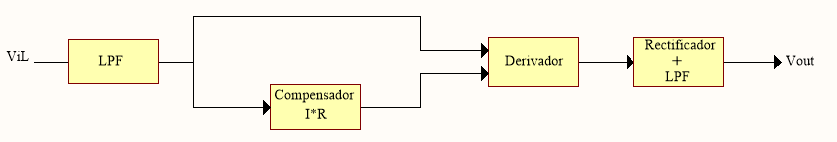
\includegraphics[scale=0.5]{Diagrama-Bloques-Estimador.png}
	\caption{Diagrama en Bloques del Estimador.}
	\label{fig:img_Diagrama-Bloques-Estimador.png}
\end{figure}

\noindent Se implementa un estimador compuesto por los bloques mostrados en la \textbf{Figura 4.14}. A este le ingresa una tensi\'{o}n triangular (ViL) que es la salida del sensor de efecto Hall. Para eliminar las componentes de alta frecuencia se aplica un filtro pasa bajos dejando pasar hasta la quinta arm\'{o}nica. Esta se\~{n}al filtrada conserva la forma triangular de la corriente. 



\noindent Al ingresar al derivador con ViL, la forma de onda resultante a su salida es aproximadamente cuadrada, y sus valores de alto y bajo se corresponden con las pendientes de bajada y subida multiplicadas por una constante de tiempo del derivador. Estas pendientes deber\'{i}an ser sim\'{e}tricas alrededor del punto de operaci\'{o}n de 2.5V, pero no lo son debido a la resistencia interna del electroim\'{a}n, que provoca que la pendiente de bajada sea mayor (en m\'{o}dulo) que la de subida. Por ello, se implementa la compensaci\'{o}n I*R, cuya salida ingresa al derivador y logra mantener la simetr\'{i}a alrededor de 2.5V. Esta se\~{n}al ingresa al \'{u}ltimo bloque que rectifica y filtra la forma de onda, obteni\'{e}ndose una tensi\'{o}n continua (Vout) proporcional a la distancia de separaci\'{o}n del gap (Yo).


\subsection{An\'{a}lisis de la estimaci\'{o}n}

\noindent La ecuaci\'{o}n que gobierna la corriente en el electroim\'{a}n se puede calcular aplicando las leyes de Kirchoff correspondientes al circuito que se ve en la \textbf{Figura 4.15.}

\begin{figure}[H]
	\centering
	\includegraphics[scale=0.9]{Circuito-electroimán-con-driver-corriente.png}
	\caption{Circuito del electroimán con el driver de corriente.}
	\label{fig:img_Circuito-electroimán-con-driver-corriente.png}
\end{figure} 

\noindent Sabiendo que$\ L(y)$ se puede aproximar como en la \textbf{ecuaci\'{o}n} \textbf{4.9}, y que $L_{\infty }$(inductancia de dispersi\'{o}n) es la inductancia del electroim\'{a}n sin la pieza en forma de ``I'' :

\begin{equation} \label{eq_inductancia_f(y)}
	L(y)\ \approx \ \mu o\frac{N^2*A}{2Y} 
\end{equation}

\begin{equation} \label{eq_VbusCondicion}
	\pm V_{BUS}-\ L(y)*\left|\frac{{di}_L}{dt}\right|-L_{\infty }*\left|\frac{{di}_L}{dt}\right|-R_L*I_L=0
\end{equation}


\noindent Asumiendo que:

\begin{equation} \label{eq_Derivadadi-dt}
	V_{BUS}>>i_L*R_L
\end{equation}
 
\noindent Se aproxima la derivada de la corriente como:

\begin{equation} \label{eq_derivadaAproximacion}
	\left|\frac{{di}_L}{dt}\right|\simeq \frac{V_{BUS}}{L(y)+L_{\infty }}=\frac{V_{BUS}}{L_T(y)}
\end{equation}

\noindent Seg\'{u}n mediciones realizadas, se tienen los valores de $L_T(y)$ correspondientes a cada posici\'{o}n. En base a ellos se hace una aproximaci\'{o}n lineal para obtener la expresi\'{o}n de la derivada de la \textbf{ecuaci\'{o}n 4}.\textbf{10.}

\noindent 

\begin{equation} \label{eq_di-dt_lineal}
{\left|\frac{{di}_L}{dt}\right|}_{Lineal}=\ 194690\ *\ Y[m]+676\ A/s
\end{equation}

\subsection{Modelo circuital del estimador de posici\'{o}n}

\noindent Para poder obtener $\left|\frac{{di}_L}{dt}\right|$ se utiliza un circuito derivador con un amplificador operacional como se observa en la \textbf{Figura 4.16}.

\begin{figure}[H]
	\centering
	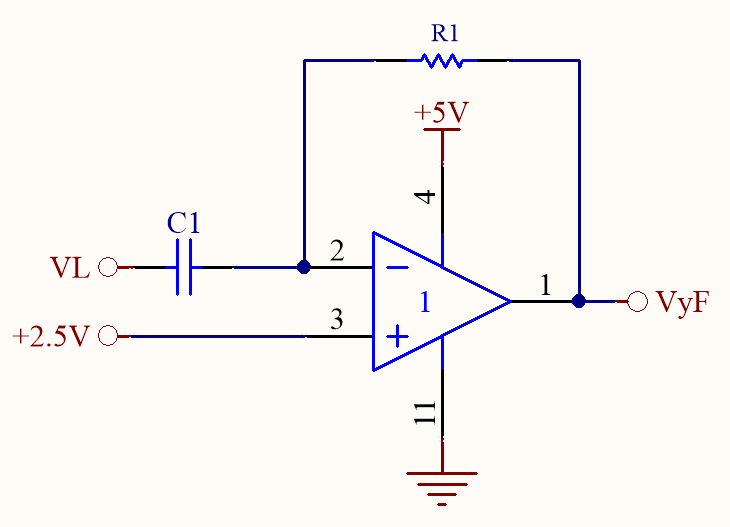
\includegraphics[scale=0.3]{Circuito-derivador.png}
	\caption{Circuito derivador.}
	\label{fig:img_Circuito-derivador}
\end{figure}

\noindent La salida del circuito, $V_{yf}(t)$, ante una entrada $V_L$ es:

\begin{equation} \label{eq_vyf1}
	V_{yf}(t)\ =\ 2.5V\ -\ \frac{dV_L}{dt}*C_1*R_1
\end{equation}


\noindent Considerando $V_L=K_h*i_L$, donde Kh es la constante del sensor de efecto Hall, se obtiene: 

\begin{equation} \label{eq_vyf2}
	V_{yf}(t)\ =2.5V\ -\frac{diL}{dt}*K_h*C_1*R_1
\end{equation}

\noindent $V_{yf}(t)$ tiene variaciones alrededor del setpoint de 2.5 V. Por lo tanto, para evitar la saturaci\'{o}n del derivador se debe cumplir que:

\begin{equation} \label{eq_vyf3}
	\left|-\frac{diL}{dt}*K_h*C_1*R_1\right|\ \le 2.5V
\end{equation}

\noindent Por lo tanto, con la ecuaci\'{o}n \ref{eq_derivadaAproximacion} y \ref{eq_di-dt_lineal}:

\begin{equation} \label{eq_condicionC1-R1}
	C_1*R_1<=\frac{2.5\ V\ *L_{min}}{V_{BUS}*K_h}
\end{equation}

\noindent Con $L_{min}=\ L_T(5\ mm)=\ 14.9\ mH$ (teniendo en cuenta la inductancia de dispersi\'{o}n) se obtiene: 

\begin{equation} \label{eq_condicionC1-R1-2}
	C_1*R_1<=\ 29.1\ ms
\end{equation}

\noindent Este derivador tendr\'{a} como salida una onda pulsada, cuyo flanco superior  es proporcional a la pendiente de bajada de la corriente en el electroim\'{a}n, y el flanco inferior es proporcional a la pendiente de subida de la corriente. 

\noindent Para los c\'{a}lculos se utiliz\'{o} $C_1*R_1=\ 25\ mS$, para dar un margen y evitar la saturaci\'{o}n del amplificador operacional.  

\noindent Usando la \textbf{ecuaci\'{o}n 4.11 }y \textbf{4.12}, y considerando una variaci\'{o}n en torno a 2.5V se obtiene:

\noindent

\begin{equation} \label{eq_Vyf-lineal}
	Vyf(y)\ =\ |Kh*C_1*R_1*di/dt)|\ +2.5V=0.2595*y(mm)+3.4V
\end{equation}

\noindent Se puede observar en la \textbf{Tabla 4.3} que para el rango de valores posibles en los que el electroim\'{a}n trabajar\'{a}, el estimador posee un rango de salida ${\mathit{\Delta}{Vyf}_{Lineal}}(5-2\ mm)=\ 0.78\ V$.

\begin{table}[H]
	\begin{center}
		\begin{tabular}{| c | c |}
			\hline
			Y[mm] & ${Vyf(y)}_{Lineal}$\\ \hline
			2 & 3.92 \\ \hline 
			3 & 4.18 \\ \hline 
			4 & 4.44 \\ \hline 
			5 & 4.7 \\ \hline 
		\end{tabular}
		\caption{Vyf en función de la posición.}
		\label{tab_Vyf_vs_y}
	\end{center}
\end{table}

\subsection{Circuito del derivador compensado}

\noindent Puesto que los circuitos derivadores pueden presentar inestabilidad a alta frecuencia, es necesario compensarlo agregando una resistencia en serie al capacitor, para que genere un cero en la transferencia de realimentaci\'{o}n

\begin{figure}[H]
	\centering
	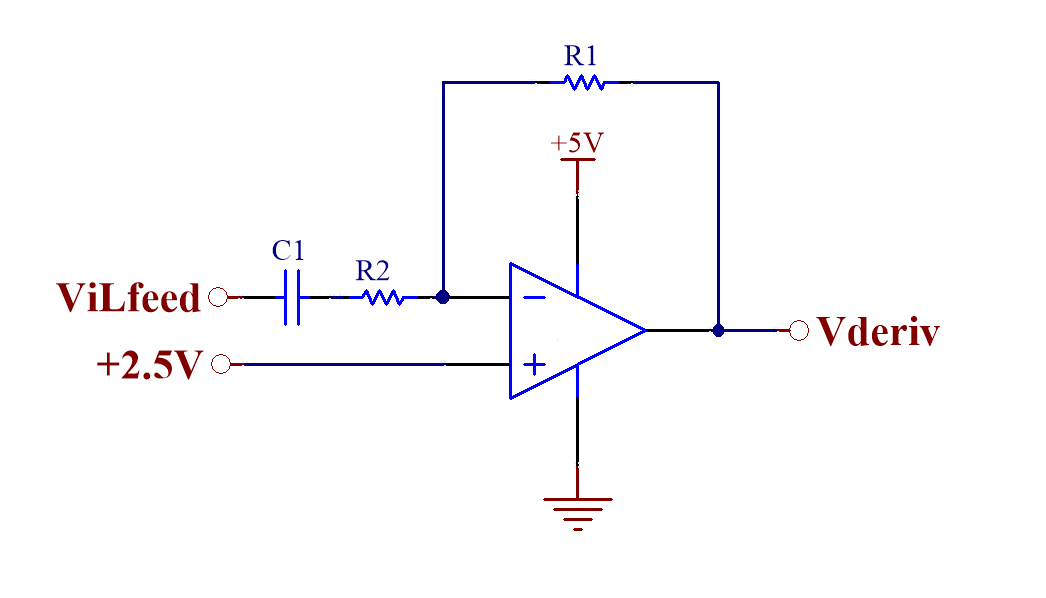
\includegraphics[scale=0.3]{Circuito-derivador- compensado.png}
	\caption{Circuito derivador compensado}
	\label{fig:img_Circuito_derivador_compensado}
\end{figure}

\noindent El operacional es internamente compensado, por lo que todos sus otros polos los tiene luego de el cruce por 0 dB de la ganancia. Para simplificar el an\'{a}lisis no se tienen en cuenta estos, ya que est\'{a}n fuera de la zona de inter\'{e}s.

\begin{equation} \label{eq_Vyf-lineal}
	A(w)=\frac{1778279}{(\frac{s}{2\pi *20}+1)}
\end{equation} 

\begin{equation} \label{eq_Vyf-lineal}
	\frac{1}{H(w)}=\frac{1+s*C_1*(R_1+R_2)}{1+s*C_1*R_2}\simeq \frac{1+s*C_1*R_1}{1+s*C_1*R_2}
\end{equation}

\noindent Para compensar el circuito se coloca un polo en 16 kHz, dando como resultado $R2=10\ ohm$, $C1=1\ uF$ y $R1=25\ kOhm\ $y un margen de fase de $\phi =49.6{}^\circ $, como se puede observar en la \textbf{Figura 4.18.}

\begin{figure}[H]
	\centering
	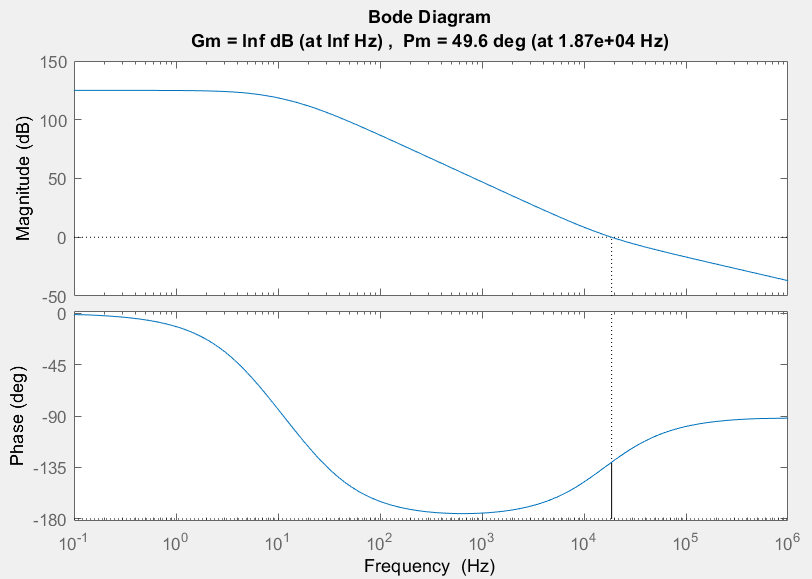
\includegraphics[scale=0.5]{GH-del-derivador-compensado.png}
	\caption{GH del derivador compensado.png}
	\label{fig:img_GH del derivador compensado}
\end{figure}

\begin{figure}[H]
	\centering
	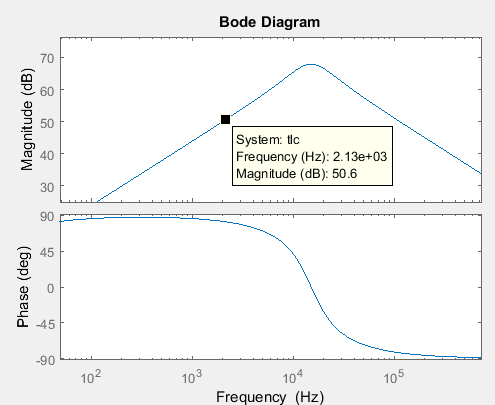
\includegraphics[scale=0.7]{Transferencia-de-lazo-cerrado.png}
	\caption{Transferencia de lazo cerrado}
	\label{fig:img_Transferencia-de-lazo-cerrado}
\end{figure}

\noindent Como se observa en la \textbf{figura 4.19, }la transferencia de lazo cerrado (TLC) tiene un comportamiento derivativo en las frecuencias cercanas a 2 kHz, como es deseado.

\noindent A continuaci\'{o}n se muestra la TLC del circuito derivador:
 
\begin{equation} \label{eq_Vyf-lineal}
	{Tlc}_{derivador}=\frac{V_{yf}}{Vil}=\frac{-0.025*s}{1+(\frac{2*0.473}{94,5\ krad/s})*s+(\frac{s}{94,5\ krad/s})^2}
\end{equation} 

\subsection{Dise\~{n}o del LPF}

\noindent Debido a que el derivador amplifica las se\~{n}ales de alta frecuencia es necesario agregar un filtro pasa bajos en su entrada. Como la se\~{n}al que va a ingresar al derivador es ViL, la cual es una onda triangular de frecuencia fundamental de 2KHz se dejar\'{a} pasar hasta la 5º arm\'{o}nica. Para su implementaci\'{o}n se utiliza un filtro activo Butterworth de orden 2, con una frecuencia de corte en 20 KHz. En la \textbf{Figura 4.20 }se puede ver el filtro utilizado y en la \textbf{Figura 4.21}, su respuesta en frecuencia.

\begin{figure}[H]
	\centering
	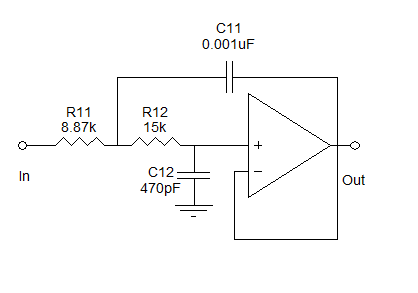
\includegraphics[scale=1]{Filtro-para-la-entrada-del-derivador.png}
	\caption{Filtro para la entrada del derivador}
	\label{fig:img_Filtro-para-la-entrada-del-derivador}
\end{figure}

\begin{figure}[H]
	\centering
	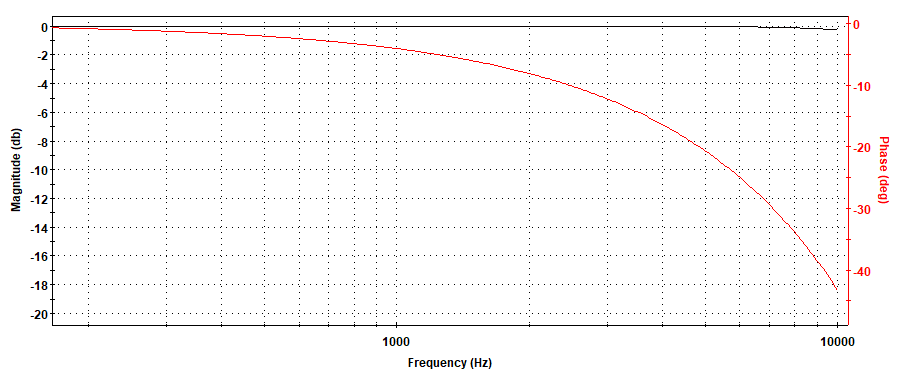
\includegraphics[scale=0.5]{Respuesta-en-frecuencia-del-filtro-activo.png}
	\caption{Respuesta en frecuencia del filtro activo}
	\label{fig:img_Respuesta-en-frecuencia-del-filtro-activo}
\end{figure}

\subsection{Compensaci\'{o}n I*R}

\noindent Al circular corriente siempre en el mismo sentido por el electroim\'{a}n, se produce una ca\'{i}da de tensi\'{o}n casi constante en la resistencia interna, haciendo que no siempre est\'{e}n aplicados $\pm 24V$ al electroim\'{a}n sino que durante el $T_{ON}$ se aplican $24V-I*R$ y durante el $T_{OFF}$ se aplican $-24V-I*R$, haciendo que las pendientes sean distintas.

\begin{equation} \label{eq_Vbus-didt-RL}
\pm V_{BUS}-L(y)*\left|\frac{{di}_L}{dt}\right|-L_{\infty }*\left|\frac{{di}_L}{dt}\right|-R_L*I_L=0
\end{equation}

\noindent C\'{o}mo  $R_L=0.2\ \mathit{\Omega}$ y suponiendo una corriente de $21\ A$

\begin{equation} \label{eq_Vbus-didt-RL-2}
\pm V_{BUS}-R_L*I_L=\ \pm 24-4.2
\end{equation}

\noindent Por lo tanto, para $V_{BUS}=24\ V$:

\begin{equation} \label{eq_Vbus-didt-RL-3}
	V_{BUS}-R_L*I_L=\ +24-4.2=\ 19.8V
\end{equation}

\noindent Para $V_{BUS}=-24\ V$

\begin{equation} \label{eq_Vbus-didt-RL-4}
	V_{BUS}-R_L*I_L=\ -24-4.2=\ 28.2V
\end{equation}

\noindent Por lo tanto, sobre el electroim\'{a}n se aplicar\'{a}n dos tensiones distintas, en valor absoluto, durante la carga y descarga. Esto provoca que la rampa de corriente sea asim\'{e}trica.

\noindent Como luego se utilizar\'{a} un rectificador de onda completa, se desea que la rectificaci\'{o}n de cada una de estas pendientes resulte en el mismo valor. En la \textbf{Figura 4.22 }se muestra el efecto luego de la rectificaci\'{o}n sin realizar ninguna compensaci\'{o}n:

\begin{figure}[H]
	\centering
	\includegraphics[scale=0.5]{Forma-de-onda-luego-de-rectificar-sin-compensación-IR.png}
	\caption{Forma de onda luego de rectificar sin compensación IR.}
	\label{fig:img_Forma-de-onda-luego-de-rectificar-sin-compensación-IR}
\end{figure}


